\documentclass[12pt]{article}
\usepackage[utf8]{inputenc} 
\usepackage{CJKutf8}        % 中文、日文、韓文包
\usepackage{hyperref}       % 超連結
\usepackage{multirow}
\usepackage{listings}       % 程式碼區塊
\usepackage{enumerate}
\usepackage{graphicx}       % 插入圖片
\usepackage{float}          % 浮點數
\usepackage{subfigure}      % 插入多圖時,用子圖顯示
\usepackage{geometry}

\geometry{a4paper, scale=0.8}
\graphicspath{{./images/}}

\title{LaTeX教學文件}
\author{Kent010341}
\date{November, 2019}
\begin{document}
	\begin{CJK*}{UTF8}{bsmi}
		\begin{titlepage}
			\maketitle
		\end{titlepage}
		\renewcommand{\contentsname}{目錄}
		\addcontentsline{toc}{section}{目錄}
		\tableofcontents
		\newpage
		
		\phantomsection
		\addcontentsline{toc}{section}{摘要}
		\renewcommand{\abstractname}{摘要}
		\begin{abstract}
			\hspace{25pt}LaTeX是一種基於TeX的排版系統,由美國電腦科學家萊斯利·蘭伯特在20世紀80年代初期開發,利用這種格式系統的處理,即使使用者沒有排版和程式設計的知識也可以充分發揮由TeX所提供的強大功能,不必一一親自去設計或校對,能在幾天,甚至幾小時內生成很多具有書籍品質的印刷品。對於生成複雜表格和數學公式,這一點表現得尤為突出。因此它非常適用於生成高印刷品質的科技和數學、物理文件。這個系統同樣適用於生成從簡單的信件到完整書籍的所有其他種類的文件。 \\
			\\
			來源:\href{https://zh.wikipedia.org/wiki/LaTeX}{維基百科}
		\end{abstract}
		\newpage
		
		\section{安裝}
			\begin{enumerate}[1.]
				\item 前往\href{https://www.texstudio.org/}{TeXstudio官網} \\ \\
				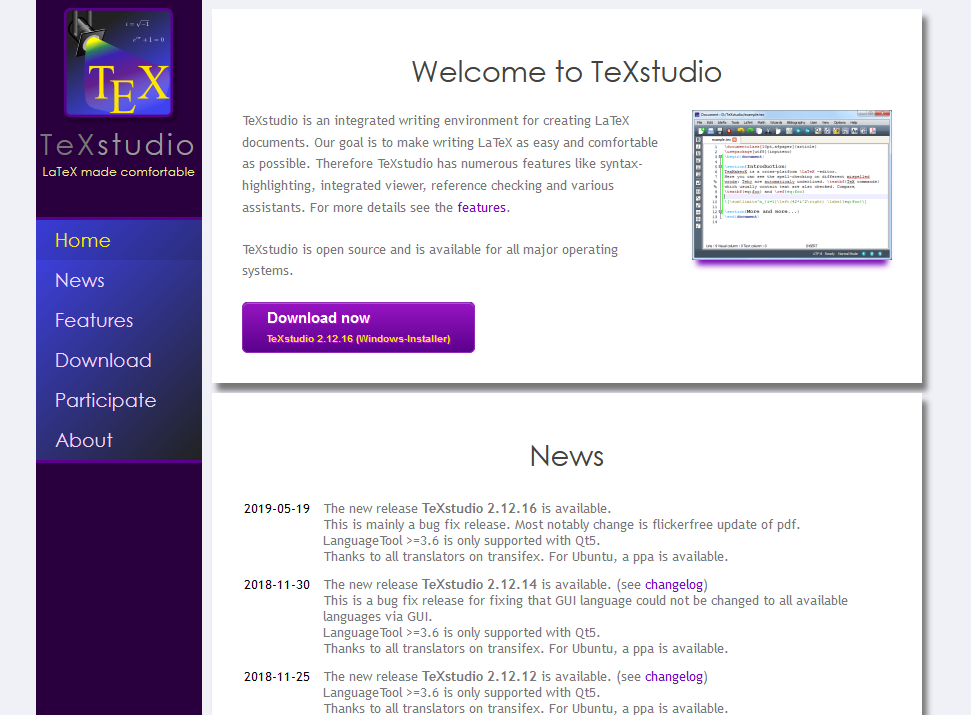
\includegraphics[scale=0.7]{TeXStudio_mainpage}
				
				\newpage
				\item 選擇對應的下載點 \\ \\
				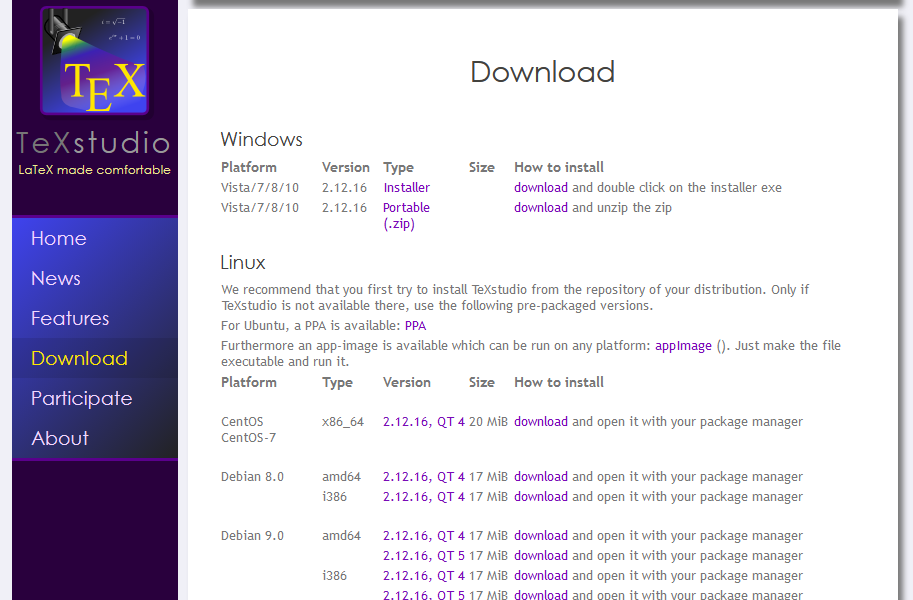
\includegraphics[scale=0.7]{TeXStudio_download}
				
				\newpage
				\item 執行安裝檔,若不須更改路徑則一路確定到底。
				\item 接著安裝MiKTeX,否則無法編譯LaTeX,\href{https://miktex.org/download}{官網連結}。 \\ \\
				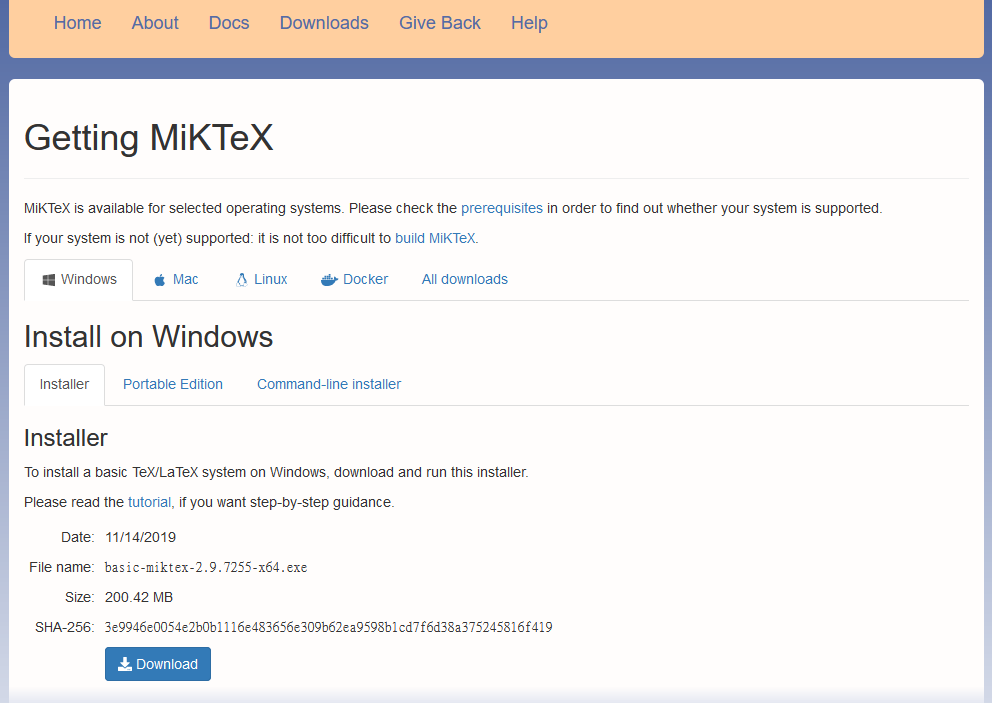
\includegraphics[scale=0.7]{MiK_download}
				\item 執行安裝檔,若不須更改路徑則一路確定到底。
			\end{enumerate}
		
		\newpage
		
		\section{TeXstudio簡介}
			\begin{itemize}
				\item 開啟TeXstudio \\ \\
				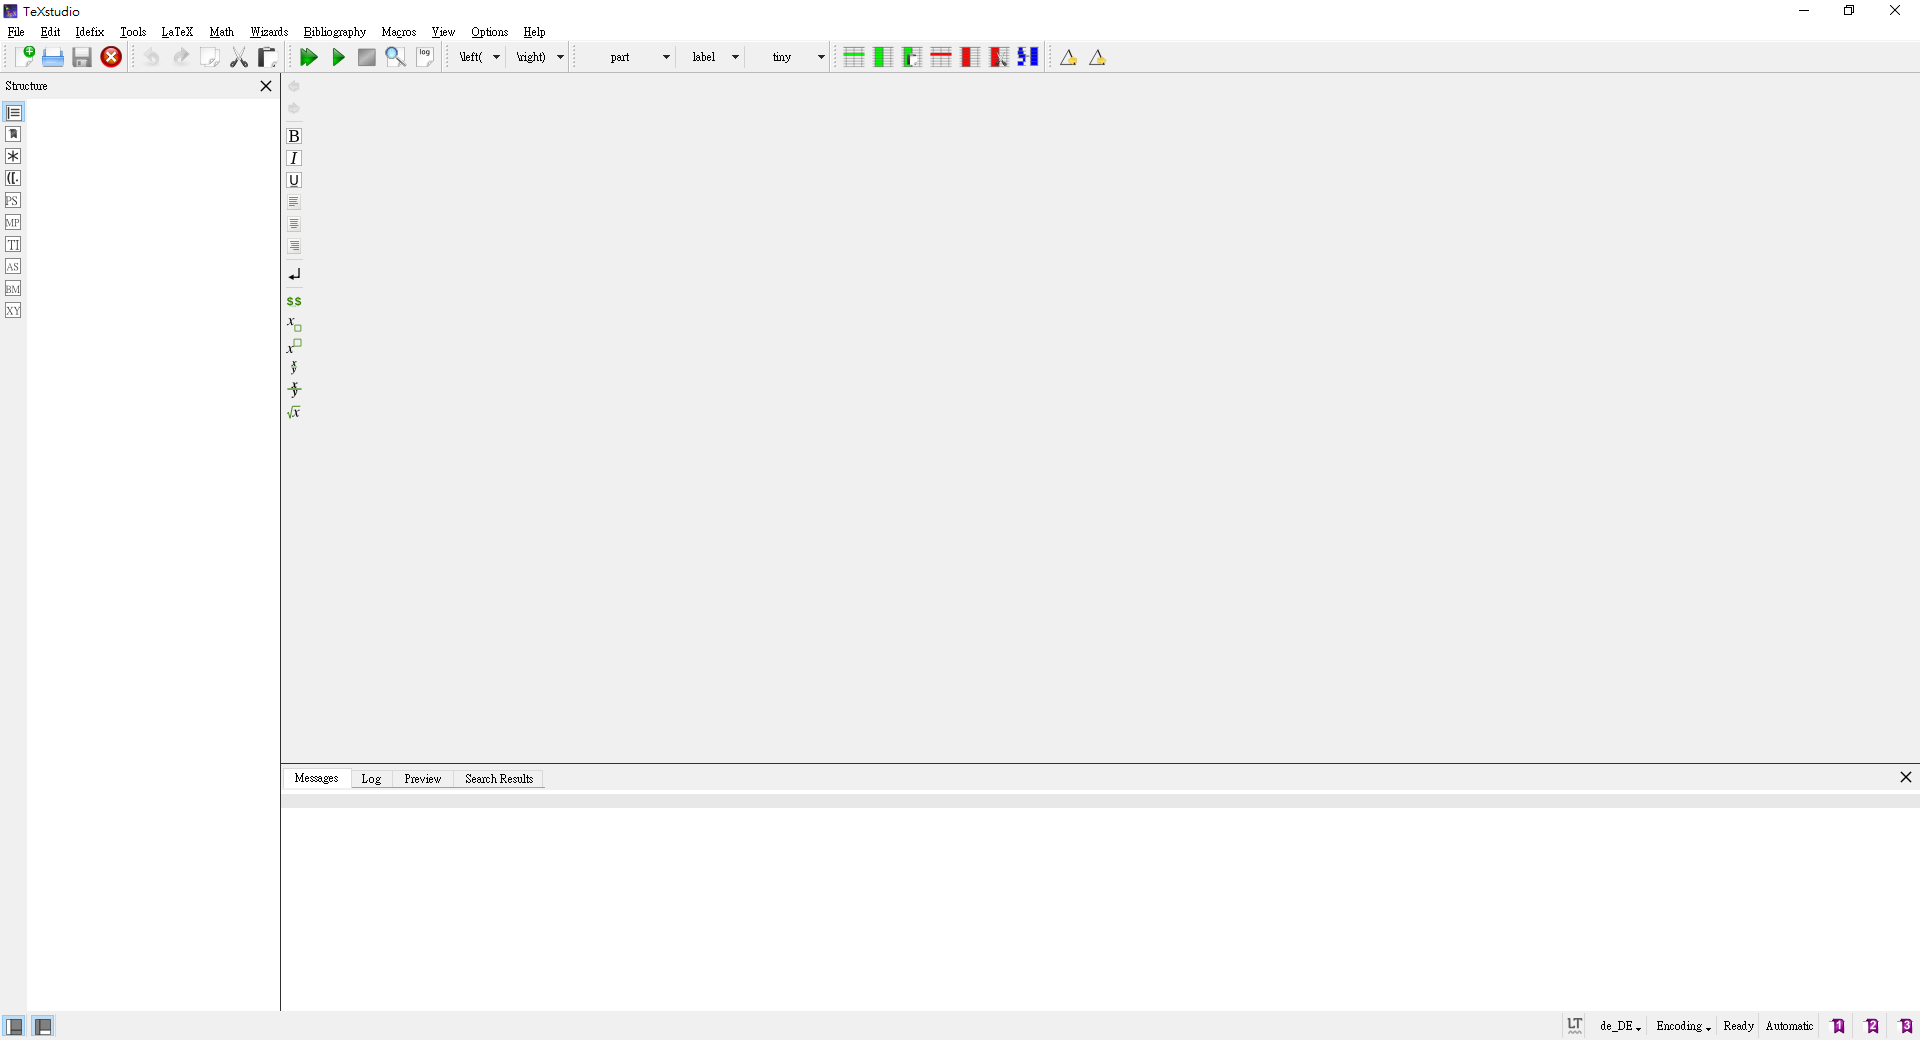
\includegraphics[scale=0.33]{TS_window}
				\item 按下新增檔案的圖示
\includegraphics[scale=1]{TS_newbtn}或Ctrl + N開新檔案。\\
				新增檔案時\textbf{建議創建新資料夾},因單一TeX檔案被編譯後會產生數個檔案。
				
				\item 按下F7開啟預覽視窗,檔案被編譯(F6)後會顯示在此視窗。 \\ \\
				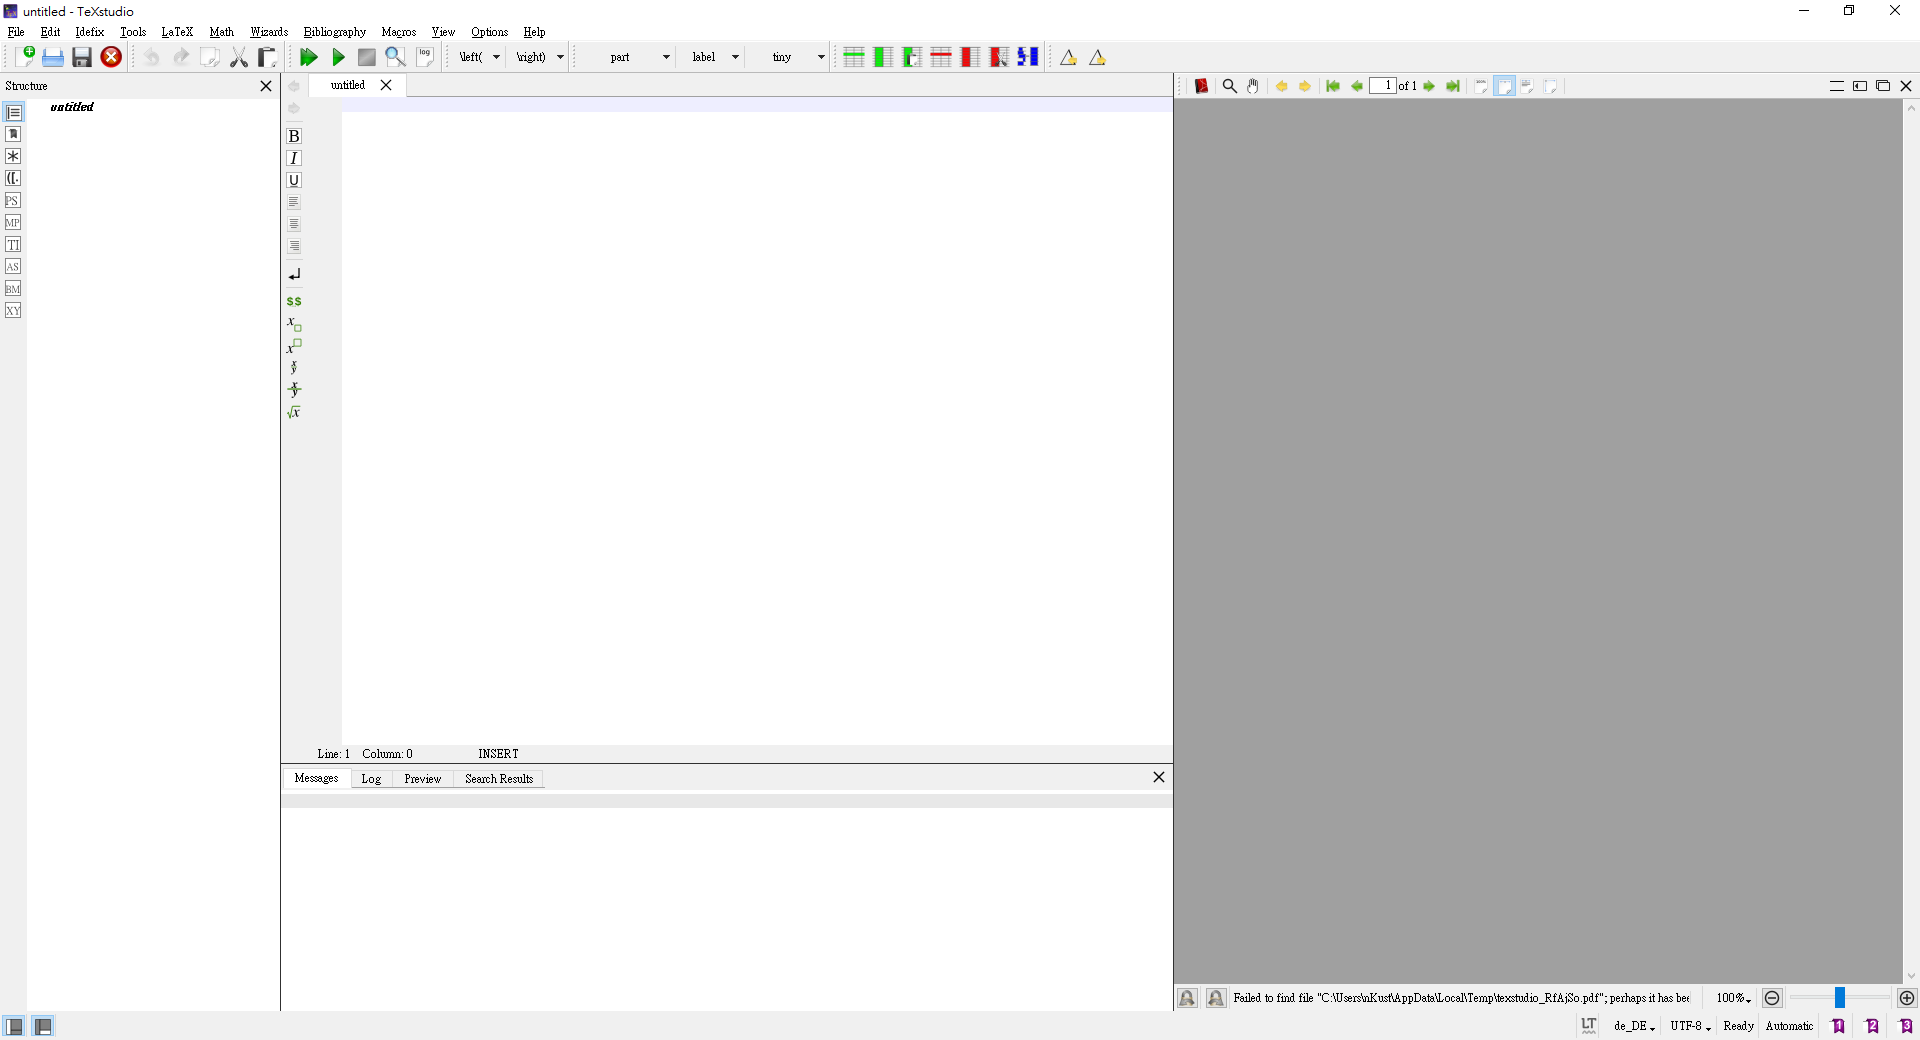
\includegraphics[scale=0.33]{TS_F7}
			\end{itemize}
			
		\newpage
		
		\section{MiKTeX簡介}
			\hspace{25pt}MiKTeX除了提供TeXstudio編譯環境,還提供了MiKTeX Console方便管理函式庫及版本更新,介面如下: \\ \\
			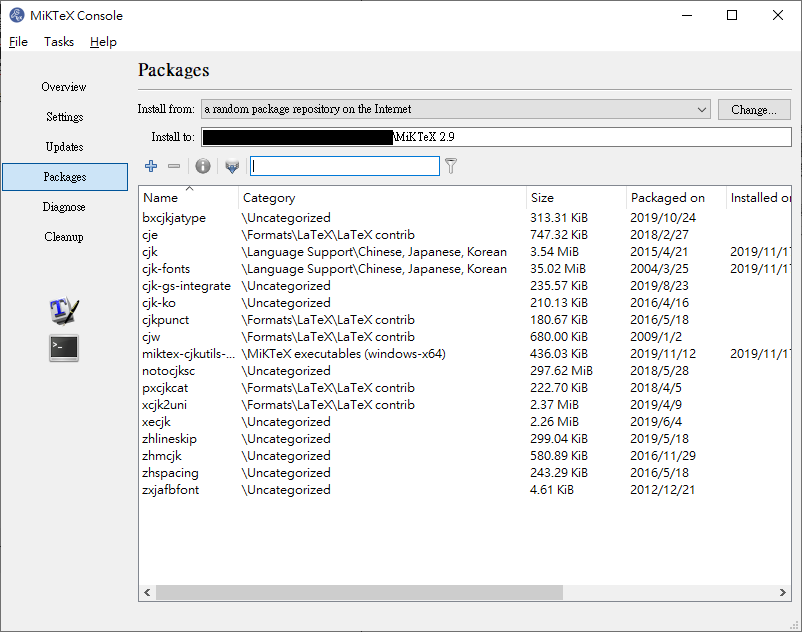
\includegraphics[scale=0.7]{MiKTeX_console} \\ \\
			\hspace{25pt}常用的是\textbf{Updates}及\textbf{Packages},Updates為版本更新,Packages則是用於下載其他函式庫,可透過搜尋找到所需函式庫。
			
		\newpage
			
		\section{LaTeX 基礎}
			\hspace{25pt}LaTeX為文件排版系統,故其與html語法非常相似。以下會說明設定一份文件常用的指令: \\
			\begin{enumerate} [1.]
				\item \textbackslash documentclass \\ \\
					在文件的一開始會定義文件的\textbf{文檔類型},使用\textbackslash documentclass:
					\begin{center}
						\textbackslash documentclass[options]\{class\}
					\end{center}
					\hspace{25pt}範例:一份文件可能會以這樣作為開頭:\textbackslash documentclass[11pt,twoside,a4paper]\{article\}。詳細說明在\href{https://zh.wikibooks.org/zh-tw/LaTeX/\%E5\%9F\%BA\%E7\%A1\%80}{維基百科}能查到。
				\item \textbackslash usepackage \\ \\
					在編輯文件過程中通常會需要透過\textbf{匯入函式庫}使用一些特殊功能,使用\textbackslash usepackage:
					\begin{center}
						\textbackslash documentclass[options]\{package\}
					\end{center}
					\hspace{25pt}範例:匯入中文函式庫:\textbackslash documentclass\{CJKutf8\}
				\item 標題、作者等文件開頭相關,更詳細在\href{https://www.overleaf.com/learn/latex/Sections_and_chapters}{此網址}。 \\ \\
					\hspace*{25pt}以下指令為非必要,當使用\textbackslash maketitle時若以下未設定則會產生預設值。
					\begin{itemize}
						\item \textbackslash title\{標題\}
						\item \textbackslash author\{作者\}
						\item \textbackslash thanks\{感謝詞\}
						\item \textbackslash date\{時間,未使用會自動產生當天\}
					\end{itemize}
			\end{enumerate}
	
		\newpage
		
		\subsection{begin及end用法}
			以下先以設定文件本文區塊為例:\\ \\
			\textbackslash begin\{document\} \\
			這裡是內文\\
			這裡也是喔\\
			\textbackslash end\{document\} \\ \\
			\hspace*{25pt}\textbackslash begin後面的\{\}間為此區塊的功能,有些功能後面會有[]放置其他參數,在後續的範例會提到。此外,一個begin一定要搭配一個end,否則會出錯。 \\ \\
			\hspace*{25pt}在上一段落提到的\textbackslash maketitle,若置於\textbackslash begin{titlepage}與對應的end間,則\textbf{文件的首頁會單獨列出}設定好的標題、作者等內容;反之若\textbackslash maketitle單獨出現,則僅會在\textbf{文件最上方}產生。 \\ \\
			至此,已經可以完成一份簡單的文件: \\ \\
				\textbackslash documentclass[12pt]\{article\} \\
				\textbackslash usepackage[utf8]\{inputenc\} \\
				\textbackslash title\{A document\} \\
				\textbackslash author\{Author A, Author B\} \\
				\textbackslash date\{November, 2019\} \\
				\textbackslash begin\{document\} \\
				\hspace*{25pt}\textbackslash begin\{titlepage\} \\
				\hspace*{50pt}\textbackslash maketitle \\
				\hspace*{25pt}\textbackslash end\{titlepage\} \\
				\hspace*{25pt}Something here \\
				\textbackslash end\{document\} 
				
			\newpage
			編譯後為:\\ \\
			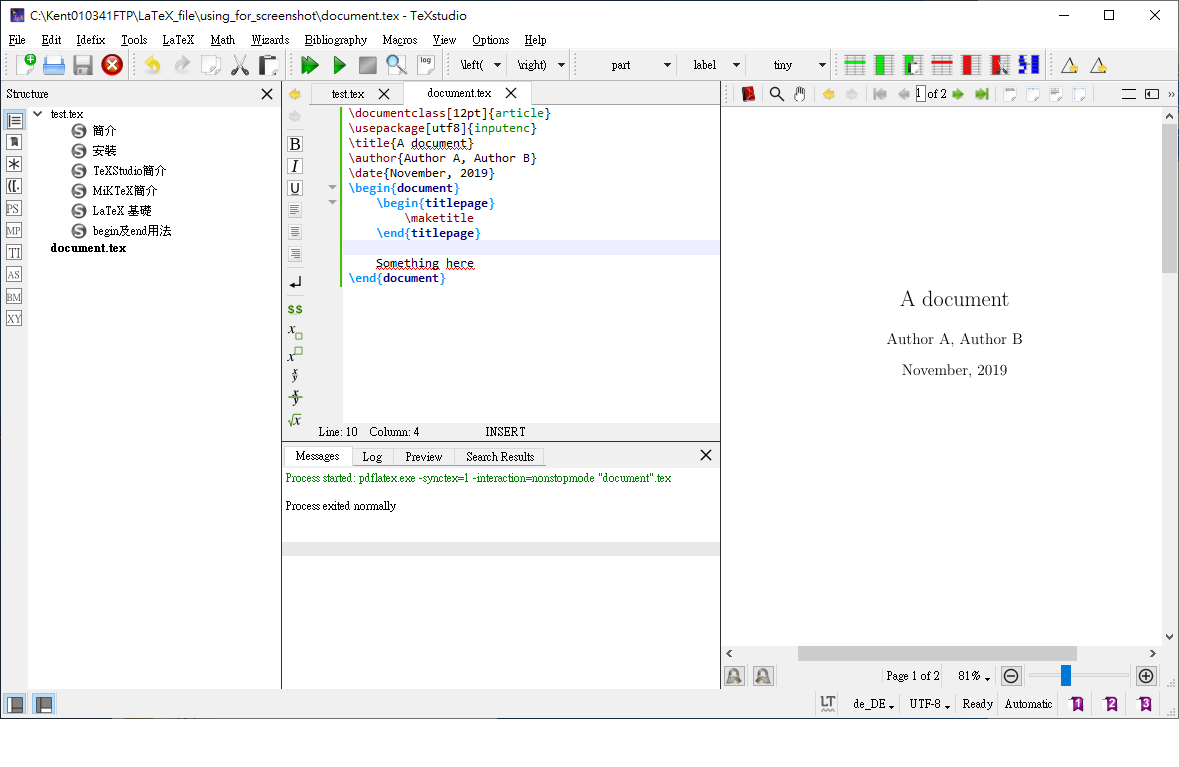
\includegraphics[scale=0.5]{easy_sample} \\
			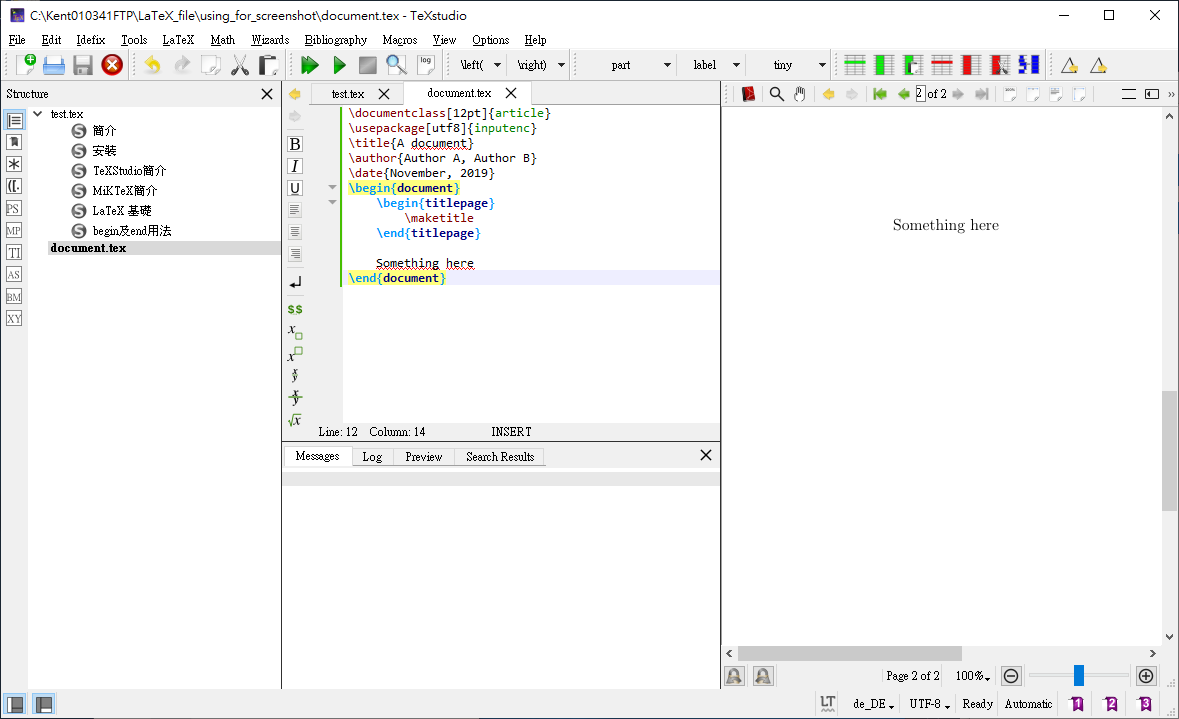
\includegraphics[scale=0.5]{easy_sample_2}
			
		\newpage
		
		\section{中文輸入}
			\hspace*{25pt}TeXstudio預設不支援編譯中文,需要安裝函式庫\textbf{cjk}才能支援中文、日文、韓文輸入。在MiKTeX console搜尋cjk,並安裝\textbf{cjk}和\textbf{cjk-fonts}: \\ \\
			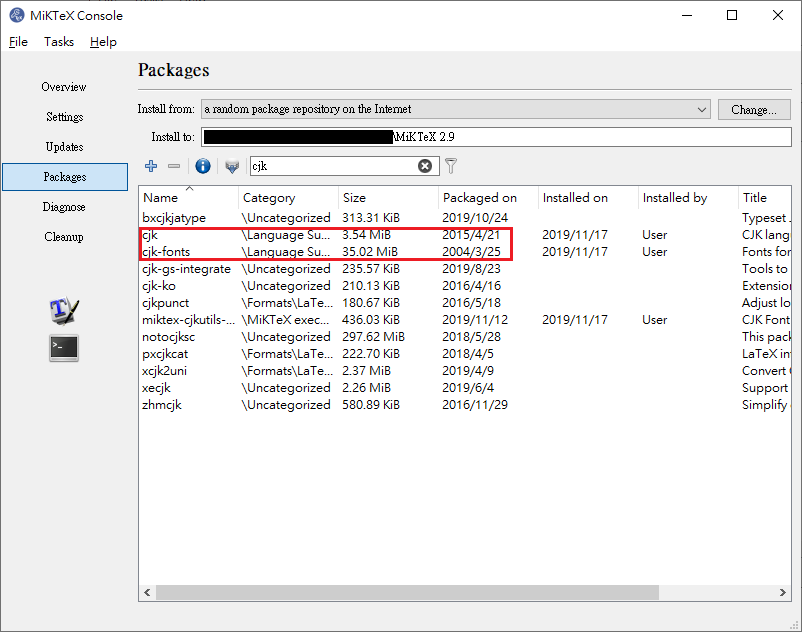
\includegraphics[scale=0.7]{MiKTeX_console_cjk}\\ \\
			接著以\textbf{\textbackslash begin\{CJK*\}\{UTF8\}\{bsmi\}}為開頭,\textbf{\textbackslash end\{CJK*\}}為結尾將需要使用中文的區塊包起即可,通常會在內文(\textbackslash begin\{document\})的內部開頭使用。
			
		\newpage
		\section{常用指令}
		
		\subsection{章節、內文相關常用指令}
			\begin{itemize}
				\item \textbf{\textbackslash chapter} \\
				創建章節,且在TeXstudio中會在左側產生快捷,方便編輯章節。\\
				article類型的文件無法使用。
				\item \textbf{\textbackslash section} \\
					創建段落,會自動標號,若不需標號則用section*。\\
					在TeXstudio中會在左側產生快捷,方便編輯章節。\\
					範例:\textbackslash section\{章節一\}
				\item \textbf{\textbackslash subsection} \\
					創建子段落,會自動標號,若不需標號則用subsection*。
				\item \textbf{\textbackslash subsubsection} \\
					創建子子段落,會自動標號,若不需標號則用subsubsection*。
				\item \textbf{\textbackslash href} \\
					超連結,需要先\textbackslash usepackage\{hyperref\}。 \\
					用法為:\textbackslash href\{連結地址\}\{顯示文字\},詳細請見\href{https://www.overleaf.com/learn/latex/Hyperlinks}{這裡}。
				\item 待更新
				
			\end{itemize}
		\subsubsection{粗體字、斜體字相關}
			\begin{itemize}
				\item 粗體:\textbackslash textbf\{文字\} \\
					效果:\textbackslash textbf\{abc\}$\Rightarrow$\textbf{abc}
				\item 斜體:\textbackslash emph\{文字\} \\
					效果:\textbackslash emph\{abc\}$\Rightarrow$\emph{abc}
				\item 下劃線:\textbackslash underline\{文字\} \\
					效果:\textbackslash underline\{abc\}$\Rightarrow$\underline{abc}
					\item 小型大寫:\textbackslash textsc\{文字\} \\
					效果:\textbackslash textsc\{abc\}DEF$\Rightarrow$\textsc{abc}DEF
			\end{itemize}
		\newpage
		
		\subsection{空白、行間距、換行、換頁}
			在LaTeX中空白、Tab、換行不具實質意義,故會有對應的指令: \\
			\begin{itemize}
				\item \textbf{\textbackslash hspace} \\
					空白,用法為\textbackslash hspace{空白大小}。\\
					空白大小支援:
					\begin{enumerate}[(1)]
						\item \textbf{pt}:英文字母單位
						\item \textbf{pc}:相當於一個中文字,1pc = 12pt
						\item \textbf{in}:英吋,1in = 72.27pt
						\item \textbf{bp}:big point,1in = 72bp
						\item \textbf{cm}:公分
						\item \textbf{mm}:毫米
						\item \textbf{em}:同\textbackslash quad
					\end{enumerate}
					範例:中文段落開頭空白為\textbackslash hspace\{2pc\}
				\item \textbf{\textbackslash quad}與\textbf{\textbackslash qquad} \\
					空白,\textbackslash qquad為比較大的空白。
				\item \textbf{\textbackslash vspace} \\
					縱向空白,即為行間距,用法\textbackslash vspace{空白大小}。
				\item \textbf{\textbackslash \textbackslash} \\
					換行。 \\
					範例:這是第一行\textbackslash \textbackslash \\
				\hspace*{3pc}這是第二行
				\item \textbf{\textbackslash newpage} \\
					換頁。
			\end{itemize}
		
		\newpage
		
		\subsection{常用區塊型功能}
			註:此處所稱之區塊型功能非正式用法,僅表示其需搭配begin與end使用。
			\begin{enumerate}[1.]
				\item \textbf{項目符號}: \\
					使用\textbf{itemize},搭配\textbf{\textbackslash item[符號字串]}使用。 \\ \\
					範例:\textbackslash begin\{itemize\} \\
					\hspace*{5pc}\textbackslash item[-] 項目 1 \textbackslash \textbackslash \\
					\hspace*{7pc} 項目1下的文字 \\
					\hspace*{5pc}\textbackslash item[-] 項目 2 \textbackslash \textbackslash \\
					\hspace*{7pc} 項目2以下的文字 \\
					\hspace*{3pc}\textbackslash end\{itemize\} \\ \\
					編譯後為:
					\begin{itemize}
						\item[-] 項目 1 \\
							項目1下的文字
						\item[-] 項目 2 \\
							項目2下的文字
					\end{itemize}
				\item \textbf{項目編號}: \\
					使用\textbf{enumerate},搭配\textbf{\textbackslash item}使用。 \\
					在\textbackslash begin\{enumerate\}後面可以中括號設定編號格式,格式中包含代表1的字元(1、I、A、a)將會在編譯後自動以對應編號取代。 \\ \\
					範例:\textbackslash begin\{enumerate\}[1.] \\
					\hspace*{5pc}\textbackslash item 項目 1 \textbackslash \textbackslash \\
					\hspace*{7pc} 項目1下的文字 \\
					\hspace*{5pc}\textbackslash item 項目 2 \textbackslash \textbackslash \\
					\hspace*{7pc} 項目2以下的文字 \\
					\hspace*{3pc}\textbackslash end\{enumerate\} \\ \\
					編譯後為:
					\begin{enumerate}[1.]
						\item 項目 1 \\
						項目1下的文字
						\item 項目 2 \\
						項目2下的文字
					\end{enumerate}
				\item \textbf{置中、置左、置右}: \\
					置中為center、置左為flushleft、置右為flushright,會將其內容自動調整。
			\end{enumerate}
		
		\newpage
		\subsection{產生目錄}
			\hspace*{2pc}在需要印出目錄的地方使用\textbf{\textbackslash tableofcontents}即會自動創建目錄,會依據目前的內文自動更新,無須手動調整。 \\ \\
			\hspace*{2pc}在論文編寫中,摘要(abstract)、致謝(thanks)、資料來源(reference)等不屬於section,不會被LaTeX加入目錄,在開頭使用
			\begin{center}
				\textbf{\textbackslash phantomsection}
			\end{center}
			新增虛構段落,並用
			\begin{center}
				\textbf{\textbackslash addcontentsline\{toc\}\{section\}\{虛構段落名稱\}} 
			\end{center}
			設定名稱,即會產生於目錄中。
		
		\newpage
		
		\section{論文編輯相關}
			\subsection{自訂標題格式}
				\href{https://zh.wikibooks.org/zh-tw/LaTeX/\%E7\%94\%9F\%E6\%88\%90\%E5\%B0\%81\%E9\%9D\%A2\%E5\%92\%8C\%E6\%A0\%87\%E9\%A2\%98}{參考資料}
			\newpage
			
			\subsection{摘要}
				\hspace*{2pc}使用\textbackslash begin\{abstract\}與\textbackslash end\{abstract\}產生摘要。
				
			\subsection{表格}
				\href{https://www.overleaf.com/learn/latex/Tables}{網路教學文件} \\
				\hspace*{2pc}表格使用\textbf{tabular}並在其後\textbf{以c代表元素置中、l置左、r置右},\textbf{$\vert$}代表格線設定框線,橫線使用\textbf{\textbackslash hline}。 \\
				\hspace*{2pc}表格元素使用\& 作為橫向的分界,\textbackslash \textbackslash 作為縱向換行。 \\ \\
				範例: \\
				\hspace*{2pc}\textbackslash begin\{tabular\}\{$\vert$l$\vert$cr$\vert$\} \\
				\hspace*{4pc} \textbackslash hline \\
				\hspace*{4pc} apple \& banana \& cat \textbackslash \textbackslash \\
				\hspace*{4pc} \textbackslash hline \\
				\hspace*{4pc} dog \& egg \& flower \textbackslash \textbackslash \\
				\hspace*{4pc} girl \& hair \& italy \textbackslash \textbackslash \\
				\hspace*{4pc} \textbackslash hline \\
				\hspace*{2pc} \textbackslash end\{tabular\} \\ \\
				編譯後為:
				\begin{tabular}{|l|cr|}
					\hline
					apple & banana & cat \\
					\hline
					dog & egg & flower \\
					girl & hair & italy \\
					\hline
				\end{tabular}
			\newpage
			\subsubsection{跨欄}
				\begin{itemize}
					\item 橫向跨欄 \\
						使用\textbf{\textbackslash multicolumn\{欄數\}\{位置與格線字串\}\{內文\}} \\ \\
						範例: \\
						\hspace*{2pc}\textbackslash begin\{tabular\}\{$\vert$l$\vert$c$\vert$r$\vert$\} \\
						\hspace*{4pc} \textbackslash hline \\
						\hspace*{4pc} \textbackslash multicolumn\{3\}\{$\vert$c$\vert$\}\{something\} \textbackslash \textbackslash \\
						\hspace*{4pc} \textbackslash hline \\
						\hspace*{4pc} apple \& banana \& cat \textbackslash \textbackslash \\
						\hspace*{4pc} dog \& egg \& flower \textbackslash \textbackslash \\
						\hspace*{4pc} girl \& hair \& italy \textbackslash \textbackslash \\
						\hspace*{4pc} \textbackslash hline \\
						\hspace*{2pc} \textbackslash end\{tabular\} \\ \\
						編譯後為:
						\begin{tabular}{|l|c|r|}
							\hline
							\multicolumn{3}{|c|}{something} \\
							\hline
							apple & banana & cat \\
							dog & egg & flower \\
							girl & hair & italy \\
							\hline
						\end{tabular}
					\item 縱向跨欄 \\
					需要\textbf{\textbackslash usepackage\{multirow\}}。 \\
					使用\textbf{\textbackslash multirow\{欄數\}\{寬度\}\{內文\}} \\ \\
					範例: \\
					\hspace*{2pc}\textbackslash begin\{tabular\}\{$\vert$c$\vert$l$\vert$c$\vert$r$\vert$\} \\
					\hspace*{4pc} \textbackslash hline \\
					\hspace*{4pc} \textbackslash multirow\{2\}\{5pc\}\{something\} \& apple \& banana \& cat \textbackslash \textbackslash \\
					\hspace*{4pc}  \& dog \& egg \& flower \textbackslash \textbackslash \\
					\hspace*{4pc}  \& girl \& hair \& italy \textbackslash \textbackslash \\
					\hspace*{4pc} \textbackslash hline \\
					\hspace*{2pc} \textbackslash end\{tabular\} \\ \\
					編譯後為:
					\begin{tabular}{|c|l|c|r|}
						\hline
						\multirow{3}{5pc}{something} & apple & banana & cat \\
						& dog & egg & flower \\
						& girl & hair & italy \\
						\hline
					\end{tabular}
				\end{itemize}
			
			\newpage
			\subsection{插入圖片}
				\href{https://www.overleaf.com/learn/latex/Inserting_Images}{網路教學文件} \\
				插入圖片所需的函式庫有: \\
				\begin{itemize}
					\item \textbackslash usepackage\{\textbf{graphicx}\}
					%\item \textbackslash usepackage\{\textbf{subfigure}\}
					\item \textbackslash usepackage\{\textbf{float}\}
				\end{itemize}
				插入圖片前可先設定圖片路徑,避免每次都輸入較長的相對路徑,故建議創建圖片專用資料夾,用以下指令設定:
				\begin{center}
					\textbf{\textbackslash graphicspath\{\{路徑\}\}}
				\end{center}
				接著使用以下指令插入圖片:
				\begin{center}
					\textbf{\textbackslash includegraphics[圖片尺寸]\{圖片路徑\}}
				\end{center}
				\begin{itemize}
					\item 圖片尺寸:可使用scale設定縮放比例、width設定寬度、height設定高度。
					\item 圖片路徑:可輸入完整路徑、相對路徑,若只輸入檔案名稱則會從先前graphicspath所設定之路徑尋找。
				\end{itemize}
				
				\subsubsection{圖片名稱及自動標號}
					使用\textbackslash begin\{figure\}與\textbackslash end\{figure\}。 \\
					範例: \\
					\hspace*{2pc}\textbackslash begin\{figure\}[h] \\
					\hspace*{4pc}\textbackslash centering \% 圖片置中\\
					\hspace*{4pc}\textbackslash includegraphics[scale=0.2]\{sin\} \% 插入圖片 \\
					\hspace*{4pc}\textbackslash caption\{a sin plot\} \% 圖片名稱 \\
					\hspace*{4pc}\textbackslash label\{fig:sum\} \% 後續可用ref取得該圖編號、名稱、所在頁數 \\
					\hspace*{2pc}\textbackslash end\{figure\} \textbackslash \textbackslash \\
					\hspace*{2pc}Figure \textbackslash ref\{fig:sin\}的名稱是\textbackslash nameref\{fig:sin\},在第\textbackslash pageref\{fig:sin\}頁。 \\
					\begin{figure}[h]
						\centering
						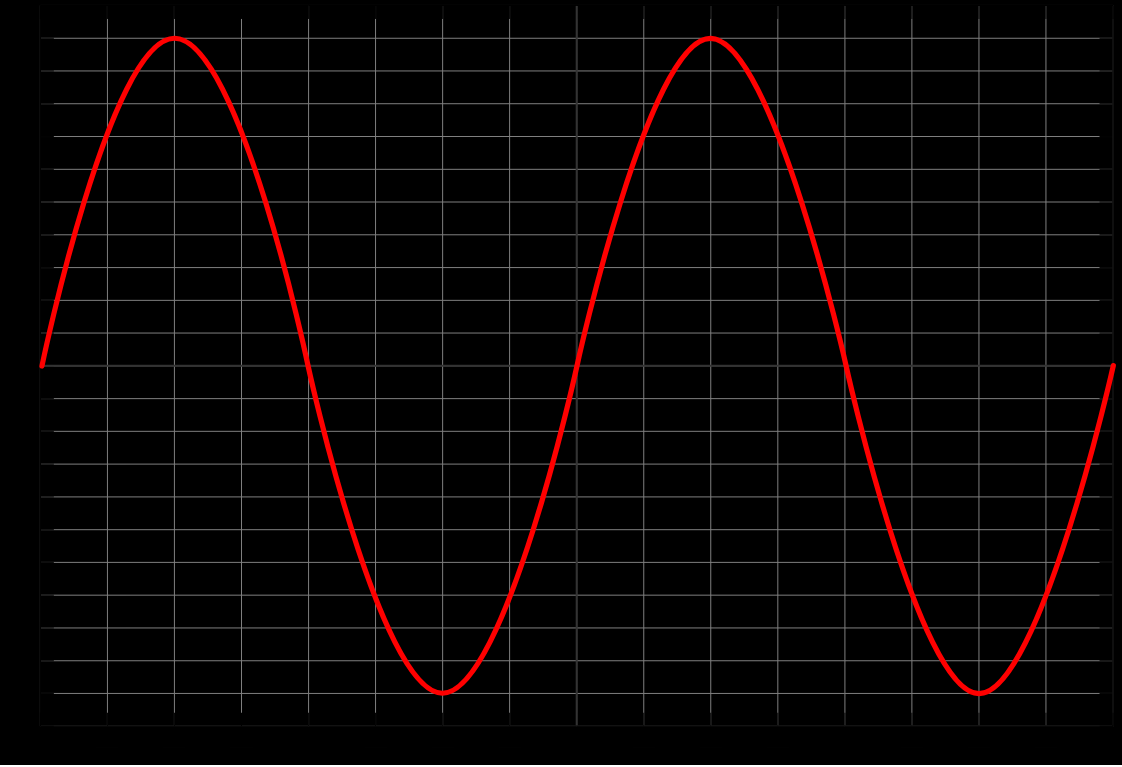
\includegraphics[scale=0.2]{sin}
						\caption{a sin plot}
						\label{fig:sin}
					\end{figure} \\
					Figure \ref{fig:sin}的名稱是\nameref{fig:sin}在第\pageref{fig:sin}頁。.
			\newpage
			\subsection{參考資料}
				\hspace*{2pc}在需要產生參考資料的地方使用\textbackslash begin\{thebibliography\}\{長度\}與\textbackslash end\{thebibliography\}。
				新增參考資料項目使用\textbackslash bibitem\{citekey\},並在其後打內容,citekey為定義此參考資料的名稱,可以在內文使用\textbackslash cite\{citekey\}建立連結與編號。
			
			\subsection{方程式}
				\href{https://codertw.com/\%E7\%A8\%8B\%E5\%BC\%8F\%E8\%AA\%9E\%E8\%A8\%80/562803/}{網路參考資料} \\
				方程式有幾種使用方式(不含自動編號式,於子章節補充):
				\begin{enumerate}[1.]
					\item 單行式:
						\begin{itemize}
							\item \$數學式\$ \\
								效果:\$x\string^2=0\$$\Rightarrow x^2=0$
							\item \textbackslash(數學式\textbackslash) \\
								效果:\textbackslash(x\string^2=0\textbackslash)\(\Rightarrow x^2=0\)
						\end{itemize}
					\item 獨立行式:
						\begin{itemize}
							\item \$\$數學式\$\$ \\
								效果:\$\$x\string^2=0\$\$$\Rightarrow$$$x^2=0$$
							\item \textbackslash[數學式\textbackslash] \\
								效果:\textbackslash[x\string^2=0\textbackslash]$\Rightarrow$\[x^2=0\]
						\end{itemize}
				\end{enumerate}
			\subsubsection{方程式自動標號}
				範例: \\
				\hspace*{2pc}\textbackslash begin\{equation\} \\
				\hspace*{4pc}x\string^2=0 \\
				\hspace*{4pc}\textbackslash label\{eq:x2\} \\
				\hspace*{2pc}\textbackslash end\{equation\} \\
				這是第\textbackslash ref\{eq:x2\}個方程式。\\ \\
				編譯後: \\
				\begin{equation}
					x^2=0
					\label{eq:x2}
				\end{equation}
				這是第\ref{eq:x2}個方程式。
				
			\subsubsection{方程式內部對齊}
				\begin{eqnarray}
					z_1&&=x^2+y^2 \\
					z_2&&=(x+3)^2+(y-4)^2
				\end{eqnarray}
			\newpage
			\subsection{變更頁面尺寸及內文邊距}
				使用\textbackslash usepackage\{\textbf{geometry}\}匯入函式庫,在檔案開頭用以下指令設定:
				\begin{center}
					\textbf{\textbackslash geometry\{options\}}
				\end{center}
				options可以使用:
				\begin{itemize}
					\item 頁面尺寸,例:a4paper、letterpaper等。
					\item scale=比例,內文站整頁的比例。
					\item left=左側邊距,right=右側邊距,top=上方邊距,bottom=下方邊距,angle設定旋轉角度。
				\end{itemize}
				範例: \\
				\begin{itemize}
					\item \textbackslash geometry\{a4paper,scale=0.8\}
					\item \textbackslash geometry\{a4paper,left=2cm,right=2cm,top=1cm,bottom=1cm\}
				\end{itemize}
			\subsection{更改預設名稱}
				預設名稱如自動產生的摘要(Abstract)、目錄(Contents)、參考資料(References)、圖片(Figure.),使用以下指令更改:
				\begin{center}
					\textbackslash renewcommand\{欲更改項目\}\{新的名稱\}
				\end{center}
				而對應的\textbf{欲更改項目}為:
				\begin{itemize}
					\item 摘要:\textbackslash abstractname
					\item 目錄:\textbackslash contentsname
					\item 參考資料:\textbackslash refname
					\item 圖片:\textbackslash figurename
				\end{itemize}
			
	\end{CJK*}
\end{document}